\documentclass{article}

\usepackage{float}
\usepackage{amsmath}
\usepackage{amsfonts}
\usepackage{amssymb}
\usepackage{graphicx}
\usepackage[margin=1in]{geometry}

\usepackage[backend=biber, style=alphabetic, sorting=ynt]{biblatex}

\title{Week 7 - Homework 4}
\author{Artur Topal, S5942128}
\date{\today}

\begin{document}

\maketitle

\begin{center}
  \textbf{TA}: Hanna, grp\_356739\_6
\end{center}

\pagebreak

\section{ Problem H1 } 
A vector field $\mathbf{F}$ is conservative if and only if $\nabla \times \mathbf{F} = \vec{0}$. Verify if that is the case for

\begin{equation}
  \mathbf{F} = (2x + y)\hat{i} + (z\cos(yz) + x)\hat{j} + y\cos(yz)\hat{k}   
\end{equation}

\begin{equation*}
  \nabla \times \mathbf{F} = \begin{vmatrix}
\hat{i} & \hat{j} & \hat{k}\\
\partial_x & \partial_y & \partial_z \\
2x+y & z\cos(yz)+x & y\cos(yz)
  \end{vmatrix} =
\end{equation*}

\begin{equation*}
  = \hat{i} \left(
    \frac{\partial}{\partial y} (y\cos(yz)) -  \frac{\partial}{\partial z} (z\cos(yz)+x)
    \right) - \hat{j} \left(
    \frac{\partial}{\partial x} (y\cos(yz)) -  \frac{\partial}{\partial z} (2x+y)
    \right) + \hat{k} \left(
    \frac{\partial}{\partial x} (z\cos(yz)+x) -  \frac{\partial}{\partial y} (2x+y)
    \right)
\end{equation*}

\begin{equation*}
  = \hat{i} \left( \left[ \cos(yz) - zy\sin(yz) \right] - \left[ \cos(yz) - zy\sin(yz) \right] \right)
  - \hat{j} \left( 0 - 0  \right)
  + \hat{k} \left( 1 - 1  \right) = \vec{0}
\end{equation*}

Since $\mathbf{F}$ is conservative, there exists a function $f(x, y, z) \in C^1$ such that $\mathbf{F} = \nabla f$. Thus we get the following set of equations:

\begin{equation} \label{eq:set}
  \begin{pmatrix}
    2x + y \\ z\cos(yz) + x \\ y\cos(yz)
  \end{pmatrix} = \begin{pmatrix}
    \frac{\partial f}{\partial x} & \frac{\partial f}{\partial y} &  \frac{\partial f}{\partial z} 
  \end{pmatrix}^T
\end{equation}

Integrate the first equation,
\begin{equation} \label{eq:f1}
  f(x, y, z) = \int (2x + y) dx = x^2 + yx + h(y, z)  
\end{equation}

Differentiate eq.~\eqref{eq:f1} with respect to $y$.
\begin{equation} \label{eq:h}
  \frac{\partial f}{\partial y} = x + \frac{\partial h(y,z)}{\partial y}
\end{equation}

Compare eq.~\eqref{eq:h} and eq.~\eqref{eq:set}:
\begin{equation*}
  \frac{\partial f}{\partial y} = x + \frac{\partial h(y,z)}{\partial y} = z\cos(yz) + x \Rightarrow h(y, z) = \int z\cos(yz) dy = \sin(yz) + g(z)
\end{equation*}

Substitute $h(y, z)$ back into eq.~\eqref{eq:f1}
\begin{equation} \label{eq:f2}
  f(x, y, z) = x^2 + yx + \sin(yz) + g(z)
\end{equation}

Differentiate eq.~\eqref{eq:f2} with respect to $z$, and compare with eq.~\eqref{eq:set} to find $g(z)$
\begin{equation*}
  \frac{\partial f}{\partial z} = y\cos(yz) + \frac{dg}{dz} \Rightarrow \frac{\partial f}{\partial z} = y\cos(yz) + \frac{dg}{dz} = y\cos(yz)
\end{equation*}

\begin{equation*}
  \Rightarrow \frac{dg}{dz} = 0 \Rightarrow g(z) = K = const
\end{equation*}

Therefore,
\begin{equation*}
  f(x, y, z) = x^2 + yx + \sin(yz) + K
\end{equation*}

\section{Problem H2}

\subsection{a}
Surface $S$ is a hollow cylinder of radius $1$ extended from $z = 0$ to $z = 1$, and, from $z = 1$ to $z = 9$, it is a hollow cone at $45$ degrees. The Stoke's boundary is composed out of two boundaries $\partial S_1$\footnote{That is, a circle $x^2 + y^2 = 81, z=9$.} and $\partial S_2$\footnote{That is, a circle $x^2 + y^2 = 1, z=0$}. This is because of the (slightly informal) definition of Stoke's boundary [1] and because the specified surface is hollow.

\begin{figure}[H]
  \centering
  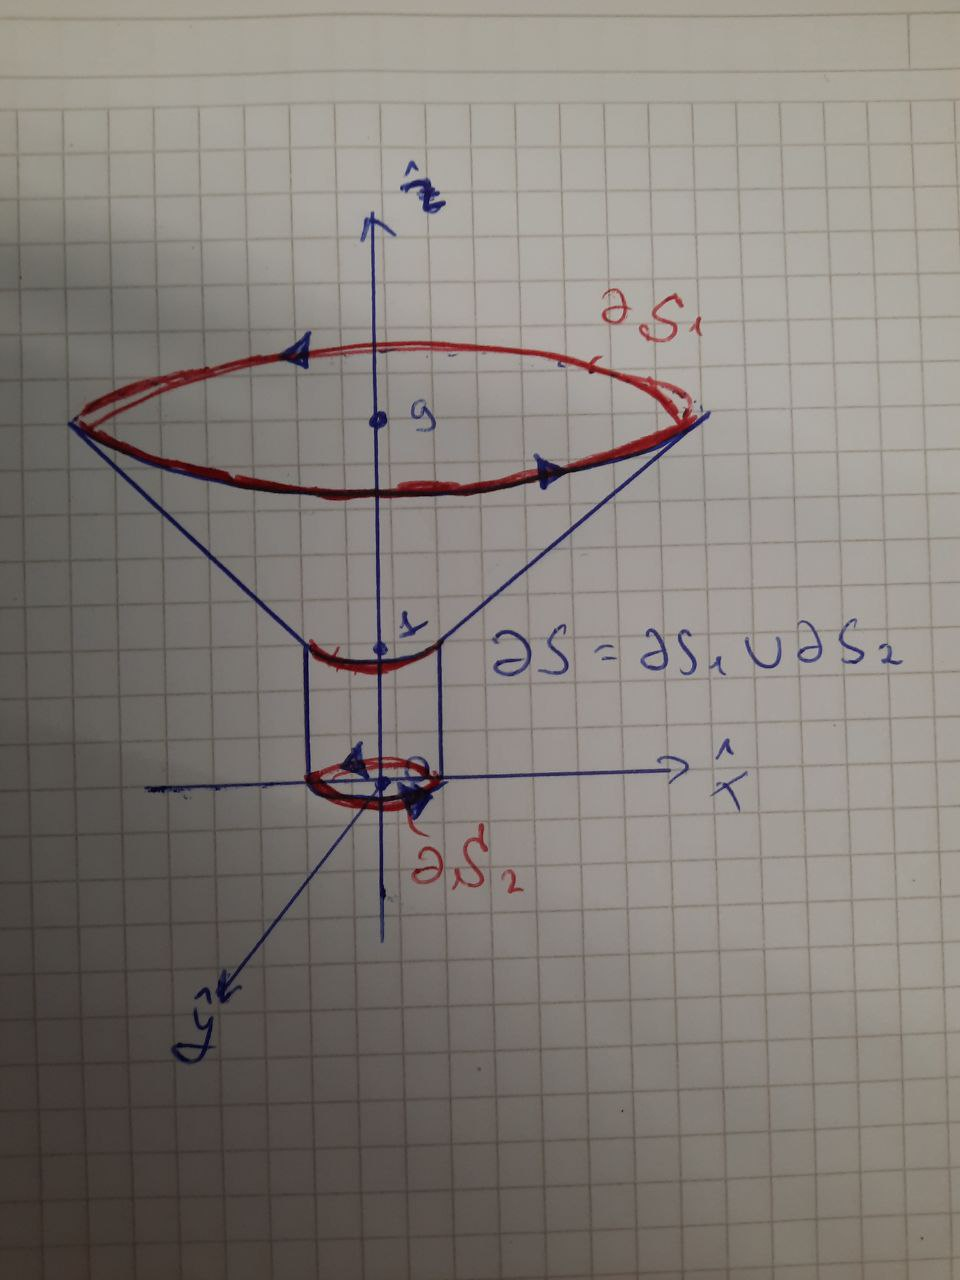
\includegraphics[width=0.3\textwidth]{calculus/W7/img/S}
  \caption{Surface S and its boundary}
  \label{fig:s}
\end{figure}

\subsection{b}
See orientation on Figure \ref{fig:s}. To find unit normal vectors to $S$, notice that $S$ is a piecewise smooth surface. Thus, $S = S_1 + S_2$ where $S_1$ is the cylinder and $S_2$ is the cone. Parametrize $S_1$ and $S_2$ 
\begin{equation*}
  S_1: \mathbf{r}(\theta, t) = \begin{pmatrix} \cos \theta \\ \sin \theta \\ t  \end{pmatrix}, D = \left\{ (t, \theta) \subset \mathbb{R} | \theta \in \left[ 0 ; 2\pi \right], t \in \left[ 0; 1 \right]  \right\}
\end{equation*}

\begin{equation*}
  S_2: \mathbf{r}(\theta, t) = \begin{pmatrix} t\cos \theta \\ t\sin \theta \\ t  \end{pmatrix}, D = \left\{ (t, \theta) \subset \mathbb{R} | \theta \in \left[ 0 ; 2\pi \right], t \in \left[ 1; 9 \right]  \right\}
\end{equation*}

Then, normal vectors are computed for each surface using $\mathbf{n} = \mathbf{r}_{\theta} \times \mathbf{r}_{t}$. For $S_1$, $\mathbf{r_\theta} = \begin{pmatrix} -\sin \theta \\ \cos \theta \\ 0  \end{pmatrix}$ and $\mathbf{r}_{t} = \begin{pmatrix} 0 \\ 0 \\ 1  \end{pmatrix}$. Therefore, the cross product is $\begin{vmatrix} \hat{i} & \hat{j} & \hat{k} \\ -\sin \theta & \cos \theta & 0 \\ 0 & 0 & 1 \end{vmatrix} = \begin{pmatrix} \cos \theta & \sin \theta & 0  \end{pmatrix}$. Therefore,
\begin{equation*}
  \mathbf{n}_{1} = \cos(\theta)\hat{i} + \sin(\theta)\hat{j}
\end{equation*}

Similarly, for $S_2$ surface, $\mathbf{r}_{\theta} = \begin{pmatrix} -t\sin \theta \\ t\cos \theta \\ 0 \end{pmatrix}$ and $\mathbf{r}_{t} = \begin{pmatrix} \cos \theta \\ \sin \theta \\ 1 \end{pmatrix}$. The cross product is
\begin{equation*}
  \mathbf{r}_{\theta} \times \mathbf{r}_{t} = 
  \begin{vmatrix}
    \hat{i} & \hat{j} & \hat{k} \\
    -t\sin \theta & t\cos \theta & 0 \\
    \cos \theta & \sin \theta & 1
  \end{vmatrix} =
  \begin{pmatrix}
    t\cos \theta \\ t\sin \theta \\ -t \sin^2 \theta - t\cos^2 \theta
  \end{pmatrix} =
  \begin{pmatrix}
    t\cos \theta \\ t\sin \theta \\ -t
  \end{pmatrix}
\end{equation*}
Thus, the normal vector to $S_2$ is
\begin{equation*}
  \mathbf{n}_{2} = t\cos(\theta)\hat{i} + t\sin(\theta)\hat{j} - t\hat{k}
\end{equation*}

$\mathbf{n}_{1}$ and $\mathbf{n}_{2}$ both point in outward direction.

\subsection{c}
Given: $\mathbf{V} = -y\hat{i} + x\hat{j} + z\hat{k}$. Since surface $S$ is not closed, the flux can be computed directly.
\begin{equation*}
  \iint_{S} \mathbf{V} \cdot d\mathbf{S} = \iint_{S_1} \mathbf{V} \cdot d\mathbf{S} + \iint_{S_2} \mathbf{V} \cdot d\mathbf{S}
\end{equation*}

\begin{equation*}
  S_1: \iint_{S_1} \mathbf{V} \cdot d\mathbf{S} =  \int_{\theta=0}^{2\pi} \int_{t=0}^{1} \mathbf{V}(\mathbf{r}(\theta, t)) \cdot (\cos(\theta)\hat{i} + \sin(\theta)\hat{j}) dtd\theta =
\end{equation*}
\begin{equation*}
  = \int_{\theta=0}^{2\pi} \int_{t=0}^{1} ( -\sin(\theta)\hat{i} + \cos(\theta)\hat{j} + t\hat{k})  \cdot (\cos(\theta)\hat{i} + \sin(\theta)\hat{j}) dtd\theta
\end{equation*}
\begin{equation*}
   = \int_{\theta=0}^{2\pi} \int_{t=0}^{1} \left( -\sin(\theta) \cos(\theta) + \cos(\theta) \sin(\theta) \right)  dtd\theta = \int_{\theta=0}^{2\pi} \int_{t=0}^{1} 0dtd\theta = 0
 \end{equation*}

\begin{equation*}
  S_2: \iint_{S_2} \mathbf{V} \cdot d\mathbf{S} = \int_{\theta=0}^{2\pi} \int_{t=1}^{9} \mathbf{V}(\mathbf{r}(\theta, t)) \cdot \mathbf{n}_{2} dtd\theta = \int_{\theta=0}^{2\pi} \int_{t=1}^{9} \begin{pmatrix} -t\sin \theta \\ t\cos \theta \\ t \end{pmatrix} \cdot \begin{pmatrix} t\cos \theta \\ t\sin \theta \\ -t \end{pmatrix} dtd\theta
\end{equation*}
\begin{equation*}
  = \int_{\theta=0}^{2\pi} \int_{t=1}^{9} \left( -t^{2}\sin \theta \cos \theta + t^{2} \sin \theta \cos \theta - t^{2}  \right)  dtd\theta = -\int_{\theta=0}^{2\pi} d\theta \int_{t=1}^{9}t^{2} dt = -2\pi \left( \frac{9^{3}}{3} - \frac{1^{3}}{3}  \right) = -\frac{1456}{3}\pi
\end{equation*}

The total flux is thus $0-\frac{1456}{3}\pi$

\textbf{Answer}: $\iint_S \mathbf{V} \cdot d\mathbf{S} = -\frac{1456}{3}\pi$
\begin{thebibliography}{99}

\bibitem{boundary}
{The Stoke's boundary}, {Toronto University, Mathematics Department}, Available: \url{https://www.math.utoronto.ca/courses/mat237y1/20189/notes/Chapter5/S5.6.html#sect-5.6.1}, Accessed: 07/01/2025.
  
\end{thebibliography}


\end{document}
